\section{Motivation}

The previous chapters developed MPC under the assumption that the prediction model used by the
controller describes the plant exactly. At each sampling instant, the controller predicts the
future evolution of the system, optimizes a finite-horizon cost, and applies the first input of the
optimal sequence. This nominal viewpoint is useful and forms the basis of the theory developed
so far, but it hides an important practical difficulty: real systems are never described perfectly
by the model used inside the optimizer.\\

Model errors may have several origins. Some parameters may be unknown or only approximately
identified, the mathematical model may neglect nonlinear effects, and the plant may be affected
by disturbances or noise. Therefore, even if the nominal prediction satisfies all constraints, the
real trajectory may deviate from it. This deviation can lead to constraint violations, degraded
performance, or even loss of feasibility of the MPC problem at later time instants.\\
Robust MPC addresses this issue by explicitly incorporating uncertainty into the control
design. The goal is no longer only to optimize the nominal predicted trajectory, but to guarantee
that the real system behaves acceptably for all admissible uncertainty realizations. In particular,
we would like the closed-loop system to satisfy constraints for all possible disturbances, to remain
stable in a suitable sense, and to retain good performance despite model mismatch.\\
A key difference with nominal MPC is that persistent disturbances generally prevent convergence
to a single equilibrium point. If the disturbance does not vanish asymptotically, then the state
cannot be expected to converge exactly to the origin. The best one can typically hope for is
convergence to a neighborhood of the origin, whose size depends on the magnitude of the
uncertainty and on the robustness properties of the controller.\\

The central question of this chapter is therefore the following. If the controller predicts the
future using a nominal model, but the real system is affected by bounded disturbances, how can
we modify the MPC formulation so that the real state still respects the constraints?

\section{Uncertainty Models}

\subsection{MPC predictions and the real system}

In nominal predictive control, the system is assumed to evolve according to a deterministic model
of the form
\[
    x(k+1) = g(x(k),u(k)).
\]
This means that, once the current state and the future input sequence are fixed, the future state
trajectory is uniquely determined. The optimizer can therefore compute a single predicted
trajectory and impose constraints directly on that trajectory.\\
In the real world, however, the evolution of the system is better described by a model of the
form
\[
    x(k+1) = g(x(k),u(k),w(k);\theta),
\]
where \(w(k)\) represents a time-varying disturbance or noise term, while \(\theta\) denotes
unknown model parameters. The disturbance \(w(k)\) changes from one sampling instant to the
next, whereas \(\theta\) is often assumed to be unknown but constant, or slowly varying. This
means that the future state is no longer uniquely determined by the current state and the planned
input sequence. Instead, each possible realization of the uncertainty gives rise to a different
trajectory.\\

This distinction is essential. In nominal MPC, one checks whether the predicted trajectory belongs
to the constraint sets. In robust MPC, one must check whether all possible trajectories generated
by the uncertainty belong to the constraint sets. Thus, the objects to be propagated are no longer
single trajectories, but sets of possible trajectories.

\subsection{Goals of robust constrained control}

Consider the uncertain constrained system
\[
    x(k+1) = g(x(k),u(k),w(k);\theta),
\]
with constraints
\[
    x(k) \in \mathcal{X}, \qquad u(k) \in \mathcal{U},
\]
and uncertainty sets
\[
    w(k) \in \mathcal{W}, \qquad \theta \in \Theta.
\]
The robust constrained control problem consists in designing a feedback law
\[
    u(k) = \kappa(x(k))
\]
such that the closed-loop system satisfies the constraints for all admissible uncertainty
realizations.\\
More precisely, the first requirement is robust constraint satisfaction:
\[
    x(k) \in \mathcal{X}, \qquad u(k) \in \mathcal{U},
    \qquad \forall k \geq 0,
\]
for all possible disturbance sequences. The second requirement is stability. Since persistent
disturbances may prevent convergence exactly to the origin, stability is usually interpreted as
convergence to a neighborhood of the origin, or as boundedness of the closed-loop trajectory in a
robust invariant region. The third requirement is performance. Depending on the available
information, one may optimize an expected cost, a worst-case cost, or a nominal cost. Finally,
one would like the controller to work from as large a set of initial states as possible.\\

These goals cannot be met without assumptions on the uncertainty. If the disturbance can be
arbitrarily large, no controller can guarantee bounded constraint satisfaction. Robust MPC
therefore requires a mathematical uncertainty model.

\subsection{Common uncertainty models}
\subsubsection{Examples of uncertainty models}
Several uncertainty models appear commonly in MPC. A first example is a constant measurement
or input bias. In this case, the dynamics may be written as
\[
    g(x(k),u(k),w(k);\theta)
    =
    \tilde g(x(k),u(k)) + \theta,
\]
where \(\theta\) is unknown but constant. Such a model is useful when the plant has a systematic
offset, for instance due to actuator bias or a constant disturbance.\\

A second important class is given by linear parameter-varying systems. In this case, the system
matrices depend on a parameter vector \(\theta(k)\), and the dynamics are written as
\[
    x(k+1)
    =
    \left(\sum_{j=0}^{n_\theta} \theta_j(k) A_j \right)x(k)
    +
    \left(\sum_{j=0}^{n_\theta} \theta_j(k) B_j \right)u(k),
\]
where
\[
    \mathbf{1}^\top \theta(k) = 1,
    \qquad
    \theta(k) \geq 0.
\]
Thus the system matrices are convex combinations of a finite number of vertex systems. This
description is useful when the dynamics vary within a known polytope of models.\\

A third possibility is additive stochastic noise:
\[
    x(k+1) = Ax(k) + Bu(k) + w(k),
\]
where the probability distribution of \(w(k)\) is known. In that case, one can formulate stochastic
MPC problems, for example by minimizing expected cost or imposing chance constraints.\\
In this chapter we focus on the deterministic robust counterpart of this last model, namely
additive bounded noise.

\subsubsection{Additive bounded noise}

The uncertainty model considered in this chapter is
\[
    x(k+1) = Ax(k) + Bu(k) + w(k),
    \qquad
    w(k) \in \mathcal{W}.
\]
Here \(A\) and \(B\) are known, while the disturbance \(w(k)\) is unknown, time-varying, and
bounded inside the set \(\mathcal{W}\). The set \(\mathcal{W}\) is assumed to contain all possible
disturbance values that may affect the system.\\
This model is simple but very important. It captures the idea that the nominal linear dynamics
are correct up to an additive perturbation. It can also be used as a conservative approximation
of more complicated effects, such as small nonlinearities, discretization errors, or unmodeled
dynamics. The price paid for this simplicity is conservatism: if \(\mathcal{W}\) is chosen too large,
the resulting robust MPC controller may become overly cautious or even infeasible for many
initial states.\\

A crucial feature of this model is that the noise is persistent. The disturbance does not
necessarily become smaller over time, and therefore the uncertain trajectory need not approach
the nominal trajectory. Instead, the possible deviation between the real and nominal trajectories
accumulates through the dynamics.

\section{Tools: Robust Invariance, Set Difference and Set Sum}

\subsection{Robust invariance and robust pre-sets}
\subsubsection{Reminder: positive invariance}
Before introducing robust invariance, we recall the nominal notion of positive invariance. Consider
an autonomous system
\[
    x(k+1) = g(x(k)),
\]
or a closed-loop system obtained by applying a fixed feedback law,
\[
    x(k+1) = g(x(k),\kappa(x(k))).
\]
A set \(\mathcal{O}\) is called positively invariant if
\[
    x(k) \in \mathcal{O}
    \quad \Longrightarrow \quad
    x(k+1) \in \mathcal{O},
    \qquad \forall k \geq 0.
\]
Thus, once the state enters \(\mathcal{O}\), it remains in \(\mathcal{O}\) forever.\\
In MPC, invariant sets are useful because they provide terminal regions in which constraint
satisfaction can be guaranteed indefinitely. If \(\mathcal{X}_f \subseteq \mathcal{X}\) is invariant
under a local controller \(\kappa\), and if \(\kappa(x) \in \mathcal{U}\) for all
\(x \in \mathcal{X}_f\), then reaching \(\mathcal{X}_f\) at the end of the prediction horizon is
sufficient to guarantee that the constraints can be respected after the horizon.

\subsubsection{Robust positive invariant sets}

In the presence of disturbances, the autonomous dynamics take the form
\[
    x(k+1) = g(x(k),w(k)),
    \qquad w(k) \in \mathcal{W}.
\]
The corresponding invariance notion must now hold for every possible disturbance.

\begin{theorembox}[Robust positive invariant set]
A set \(\mathcal{O}_{\mathcal{W}}\) is called a robust positive invariant set for
\[
    x(k+1) = g(x(k),w(k)), \qquad w(k) \in \mathcal{W},
\]
if
\[
    x \in \mathcal{O}_{\mathcal{W}}
    \quad \Longrightarrow \quad
    g(x,w) \in \mathcal{O}_{\mathcal{W}}
    \qquad \forall w \in \mathcal{W}.
\]
\end{theorembox}

The difference from nominal invariance is the universal quantifier over the disturbance. In the
nominal case, the next state must remain in the set under one deterministic successor. In the
robust case, every possible successor generated by the disturbance must remain in the set.\\
For a closed-loop system
\[
    x(k+1) = g(x(k),\kappa(x(k)),w(k)),
\]
the definition is applied to the autonomous disturbed dynamics induced by the controller
\(\kappa\). A robust invariant terminal set therefore guarantees that, once the state reaches that
set, the controller can keep the state inside it despite all admissible disturbances.

\subsubsection{Robust pre-sets}

The robust pre-set is the backward-reachability object associated with robust invariance. Given a
target set \(\Omega\), the robust pre-set is the set of all states from which the next state belongs
to \(\Omega\) for every disturbance value:
\[
    \operatorname{pre}_{\mathcal{W}}(\Omega)
    :=
    \{x \mid g(x,w) \in \Omega \ \text{for all } w \in \mathcal{W}\}.
\]
Thus, \(x \in \operatorname{pre}_{\mathcal{W}}(\Omega)\) means that no matter which admissible
disturbance occurs at the next step, the successor state is guaranteed to lie in \(\Omega\).\\
This definition is the robust counterpart of the nominal pre-set. The nominal pre-set only asks
whether the deterministic successor lies in the target set. The robust pre-set asks whether the
entire set of possible successors lies in the target set.

\subsubsection{Robust pre-sets for linear systems}

Consider now the linear disturbed system
\[
    x(k+1) = Ax(k) + w(k),
    \qquad w(k) \in \mathcal{W},
\]
and let the target set be the polyhedron
\[
    \Omega := \{x \in \R^n \mid Fx \leq f\}.
\]
The robust pre-set is
\[
\begin{aligned}
    \operatorname{pre}_{\mathcal{W}}(\Omega)
    &=
    \{x \mid Ax+w \in \Omega,\ \forall w \in \mathcal{W}\}  \\
    &=
    \{x \mid F(Ax+w) \leq f,\ \forall w \in \mathcal{W}\}  \\
    &=
    \{x \mid FAx + Fw \leq f,\ \forall w \in \mathcal{W}\}.
\end{aligned}
\]
For each row \(F_i\) of \(F\), the condition becomes
\[
    F_iAx + F_iw \leq f_i
    \qquad \forall w \in \mathcal{W}.
\]
This is equivalent to requiring the inequality to hold for the worst possible disturbance in the
direction \(F_i\):
\[
    F_iAx \leq f_i - \max_{w \in \mathcal{W}} F_iw.
\]
Therefore,
\[
    \operatorname{pre}_{\mathcal{W}}(\Omega)
    =
    \left\{
    x \ \middle|\ 
    FAx \leq f - h_{\mathcal{W}}(F)
    \right\},
\]
where \(h_{\mathcal{W}}\) denotes the support function of \(\mathcal{W}\), applied row-wise:
\[
    h_{\mathcal{W}}(F)_i
    :=
    \max_{w \in \mathcal{W}} F_iw.
\]

\begin{figure}[t]
    \centering

    \begin{subfigure}[t]{0.48\textwidth}
        \centering
        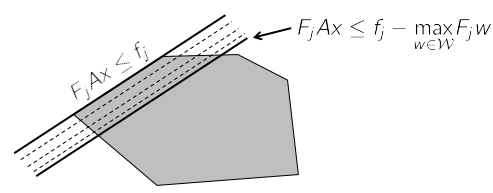
\includegraphics[width=\textwidth]{images/robust_preset_halfspace.png}
        \caption{Tightening of one supporting halfspace of the target set.}
        \label{fig:robust_preset_halfspace}
    \end{subfigure}
    \hfill
    \begin{subfigure}[t]{0.48\textwidth}
        \centering
        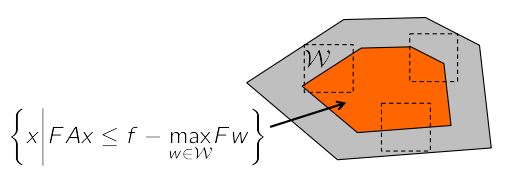
\includegraphics[width=\textwidth]{images/robust_preset_polytope.png}
        \caption{Robust pre-set obtained after tightening all inequalities.}
        \label{fig:robust_preset_polytope}
    \end{subfigure}

    \caption{Geometric interpretation of the robust pre-set for the disturbed linear system
    \(x(k+1)=Ax(k)+w(k)\). Each inequality \(F_jx\le f_j\) defining the target set
    \(\Omega=\{x\mid Fx\le f\}\) is tightened by the worst-case disturbance in the
    corresponding normal direction, leading to
    \(F_jAx\le f_j-\max_{w\in\mathcal W}F_jw\). Applying this row-wise gives
    \(\operatorname{pre}_{\mathcal W}(\Omega)
    =
    \{x\mid FAx\le f-h_{\mathcal W}(F)\}\).}
    \label{fig:robust_preset_computation}
\end{figure}

This formula is one of the central algebraic tools of robust MPC. It shows that robust
constraint satisfaction can be converted into nominal constraint satisfaction with tightened
right-hand sides. The amount of tightening is determined by the support function of the
disturbance set.

\subsubsection{Geometric condition for robust invariance}

Robust invariance can be expressed through robust pre-sets exactly as in the nominal case.

\begin{theorembox}[Geometric condition for robust invariance]
A set \(\mathcal{O}_{\mathcal{W}}\) is robust positively invariant for
\[
    x(k+1) = g(x(k),w(k)), \qquad w(k) \in \mathcal{W},
\]
if and only if
\[
    \mathcal{O}_{\mathcal{W}}
    \subseteq
    \operatorname{pre}_{\mathcal{W}}(\mathcal{O}_{\mathcal{W}}).
\]
\end{theorembox}

\begin{figure}[t]
    \centering
    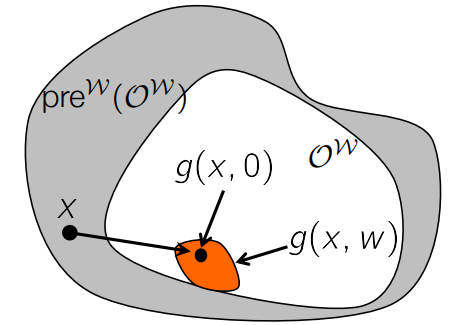
\includegraphics[width=0.48\textwidth]{images/robust_invariance_geometric_condition.png}
    \caption{Geometric interpretation of the condition
    \(\mathcal{O}_{\mathcal W} \subseteq \operatorname{pre}_{\mathcal W}(\mathcal{O}_{\mathcal W})\).
    The white region represents the set \(\mathcal O_{\mathcal W}\), while the gray region
    represents its robust pre-set \(\operatorname{pre}_{\mathcal W}(\mathcal O_{\mathcal W})\).
    For a state \(x\) to belong to the robust pre-set, all possible successors
    \(g(x,w)\), for \(w\in\mathcal W\), must remain inside \(\mathcal O_{\mathcal W}\).
    The orange set illustrates the collection of possible successor states generated by the
    admissible disturbances. Since this whole set lies inside \(\mathcal O_{\mathcal W}\),
    the point \(x\) belongs to \(\operatorname{pre}_{\mathcal W}(\mathcal O_{\mathcal W})\).}
    \label{fig:robust_invariance_geometric_condition}
\end{figure}

The interpretation is direct. If every point of \(\mathcal{O}_{\mathcal{W}}\) belongs to the robust
pre-set of \(\mathcal{O}_{\mathcal{W}}\), then every point in the set is mapped back into the set
for all admissible disturbances. Figure~\ref{fig:robust_invariance_geometric_condition}
illustrates this idea geometrically: a state belongs to the robust pre-set if the entire set of
possible one-step successors remains inside \(\mathcal O_{\mathcal W}\).

Conversely, if there exists a point in \(\mathcal{O}_{\mathcal{W}}\) that is not in the robust
pre-set, then some admissible disturbance drives the successor outside \(\mathcal{O}_{\mathcal{W}}\),
and the set is not robust invariant.

\subsubsection{Computing robust invariant sets}

The maximal robust invariant set can be computed conceptually through an iterative procedure.
Starting from the constraint set,
\[
    \Omega_0 := \mathcal{X},
\]
one recursively removes all states from which the next state cannot be guaranteed to remain in
the current candidate set:
\[
    \Omega_{i+1}
    :=
    \operatorname{pre}_{\mathcal{W}}(\Omega_i) \cap \Omega_i.
\]
The sequence is nested:
\[
    \Omega_{i+1} \subseteq \Omega_i.
\]
At each iteration, the set is made smaller by discarding states that may leave the current set
under some admissible disturbance. If the sequence reaches a fixed point,
\[
    \Omega_{i+1} = \Omega_i,
\]
then the algorithm has found a robust positively invariant set. In fact, under the usual
conditions, the fixed point is the maximal robust positively invariant subset of
\(\mathcal{X}\).

\begin{theorembox}[Conceptual algorithm for a robust invariant set]
Initialize
\[
    \Omega_0 \leftarrow \mathcal{X}.
\]
For \(i=0,1,2,\ldots\), compute
\[
    \Omega_{i+1}
    \leftarrow
    \operatorname{pre}_{\mathcal{W}}(\Omega_i) \cap \Omega_i.
\]
If
\[
    \Omega_{i+1}=\Omega_i,
\]
return
\[
    \mathcal{O}_{\mathcal{W},\infty}=\Omega_i.
\]
\end{theorembox}

This is the same algorithm used in the nominal case, with the ordinary pre-set replaced by the
robust pre-set. The robust version is more conservative because a state is kept only if all
possible disturbed successors remain admissible.\\

The distinction between nominal and robust invariance is illustrated by the closed-loop disturbed
system
\[
    x(k+1) = (A+BK)x(k) + w(k),
\]
with
\[
    A =
    \begin{bmatrix}
        1 & 1 \\
        0 & 1
    \end{bmatrix},
    \qquad
    B =
    \begin{bmatrix}
        1 \\
        0.5
    \end{bmatrix},
\]
and constraints
\[
    \mathcal{X}
    =
    \{x \mid \norm{x}_\infty \leq 5,\ \norm{Kx}_\infty \leq 1\},
    \qquad
    \mathcal{W}
    =
    \{w \mid \norm{w}_\infty \leq 0.3\}.
\]
Here \(K\) is chosen as an LQR controller. If one ignores the disturbance and computes the
maximal nominal invariant set, one obtains a region in which the nominal closed-loop trajectory
remains feasible. However, this set is not necessarily safe for the disturbed system. A state may
belong to the nominal invariant set and still be driven outside the constraints by an admissible
disturbance.

The maximal robust invariant set is therefore smaller. It contains only those states for which
the entire disturbance tube remains inside the constraints. This shrinking is not a defect of the
method; it is the price paid for a guarantee that holds for all disturbances in
\(\mathcal{W}\).

\begin{figure}[t]
    \centering
    % Replace the file name with the corresponding slide/image file.
    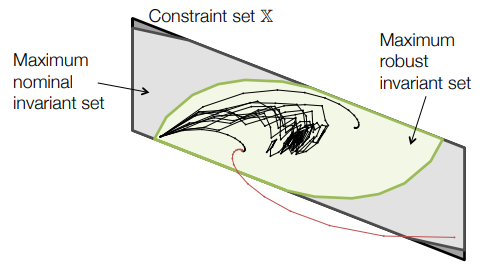
\includegraphics[width=0.5\textwidth]{images/nominal_vs_robust_invariant_set.png}
    \caption{Comparison between the constraint set, the maximal nominal invariant set, and the
    maximal robust invariant set. Robust invariance requires safety for all disturbance
    realizations, and therefore leads to a smaller admissible set.}
    \label{fig:nominal_vs_robust_invariant_set}
\end{figure}

\subsection{Minkowski sum and Pontryagin difference}

To describe robust constraint tightening compactly, two set operations are especially useful:
the Minkowski sum and the Pontryagin difference.

\begin{theorembox}[Minkowski sum]
Let \(\mathcal{A},\mathcal{B} \subseteq \R^n\). Their Minkowski sum is
\[
    \mathcal{A} \oplus \mathcal{B}
    :=
    \{x+y \mid x \in \mathcal{A},\ y \in \mathcal{B}\}.
\]
\end{theorembox}

The Minkowski sum describes all possible sums of one element from \(\mathcal{A}\) and one
element from \(\mathcal{B}\). In robust MPC, it naturally appears when adding the nominal state
to the possible disturbance offsets.

\begin{theorembox}[Pontryagin difference]
Let \(\mathcal{A},\mathcal{B} \subseteq \R^n\). Their Pontryagin difference is
\[
    \mathcal{A} \ominus \mathcal{B}
    :=
    \{x \mid x+e \in \mathcal{A}\ \text{for all } e \in \mathcal{B}\}.
\]
\end{theorembox}

The Pontryagin difference is a constraint-tightening operation. If
\[
    x \in \mathcal{A} \ominus \mathcal{B},
\]
then adding any element of \(\mathcal{B}\) to \(x\) still keeps the result inside
\(\mathcal{A}\). Therefore, if \(\mathcal{B}\) represents the set of possible errors between the
real and nominal state, then imposing
\[
    x_{\mathrm{nom}} \in \mathcal{A} \ominus \mathcal{B}
\]
guarantees
\[
    x_{\mathrm{nom}} + e \in \mathcal{A}
    \qquad \forall e \in \mathcal{B}.
\]

\begin{figure}[t]
    \centering
    % Replace the file name with the corresponding slide/image file.
    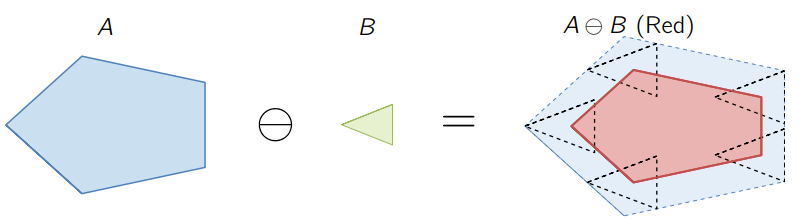
\includegraphics[width=0.70\textwidth]{images/minkowski_sum_pontryagin_difference.png}
    \caption{The Pontryagin difference tightens a set so that all admissible additions remain feasible.}
    \label{fig:minkowski_pontryagin}
\end{figure}

\section{Impact of Bounded Additive Noise}

\subsection{Uncertain state evolution}
\subsubsection{Set-valued state evolution}
We now return to the uncertain linear system
\[
    x(k+1) = Ax(k) + Bu(k) + w(k),
    \qquad w(k) \in \mathcal{W}.
\]
Given the current state \(x(0)=x_0\) and a planned input sequence
\[
    U := \{u_0,u_1,\ldots,u_{N-1}\},
\]
the future state is not a single point, because it depends on the unknown disturbance sequence
\[
    W := \{w_0,w_1,\ldots,w_{N-1}\}.
\]
We denote by
\[
    \phi_i(x_0,U,W)
\]
the state reached at time \(i\) when starting from \(x_0\), applying the input sequence \(U\),
and observing the disturbance sequence \(W\).\\
For a fixed input sequence, each possible disturbance realization produces a different trajectory.
Thus, at time \(i\), the controller must reason about a set of possible states rather than a
single predicted state.

\begin{figure}[t]
    \centering
    % Replace the file name with the corresponding slide/image file.
    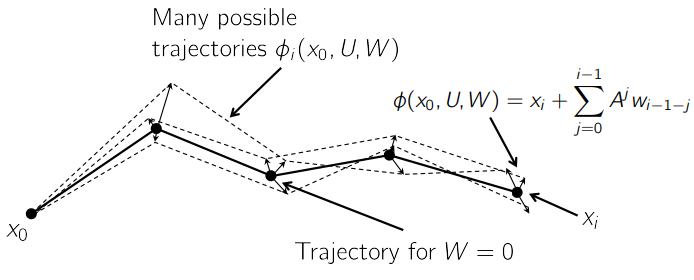
\includegraphics[width=0.6\textwidth]{images/uncertain_state_evolution.png}
    \caption{Under additive disturbances, a fixed input sequence gives rise to many possible
    trajectories. The nominal trajectory corresponds to the special case \(W=0\).}
    \label{fig:uncertain_state_evolution}
\end{figure}

\subsubsection{Nominal and uncertain predictions}

For the nominal system
\[
    x(k+1)=Ax(k)+Bu(k),
\]
successive substitution gives
\[
    x_1 = Ax_0 + Bu_0,
\]
\[
    x_2 = A^2x_0 + ABu_0 + Bu_1,
\]
and, in general,
\[
    x_i
    =
    A^i x_0
    +
    \sum_{j=0}^{i-1} A^j B u_{i-1-j}.
\]
For the uncertain system
\[
    x(k+1)=Ax(k)+Bu(k)+w(k),
\]
the first steps are
\[
    \phi_1 = Ax_0 + Bu_0 + w_0,
\]
\[
    \phi_2 = A^2x_0 + ABu_0 + Bu_1 + Aw_0 + w_1.
\]
Continuing in the same way yields
\[
    \phi_i(x_0,U,W)
    =
    A^i x_0
    +
    \sum_{j=0}^{i-1} A^j B u_{i-1-j}
    +
    \sum_{j=0}^{i-1} A^j w_{i-1-j}.
\]
Using the nominal prediction \(x_i\), this can be written compactly as
\[
    \phi_i(x_0,U,W)
    =
    x_i
    +
    \sum_{j=0}^{i-1} A^j w_{i-1-j}.
\]
Therefore, the uncertain state is equal to the nominal state plus an additive offset caused by
the accumulated disturbances.\\
This decomposition follows from linearity and is the key observation behind constraint
tightening. The nominal part depends on the chosen input sequence. The disturbance offset
depends only on the disturbance set and on the powers of \(A\).

\subsection{Robust constrained control under bounded additive noise}

\subsubsection{Goals under bounded additive noise}
We now return to the robust constrained control problem for the uncertain linear system
\[
    x(k+1) = Ax(k) + Bu(k) + w(k),
    \qquad
    x(k) \in \mathcal X,\quad u(k)\in\mathcal U,\quad w(k)\in\mathcal W.
\]
The objective is to design a feedback law
\[
    u(k)=\kappa(x(k))
\]
such that the closed-loop system satisfies the constraints for all possible disturbance
realizations, remains stable in an appropriate robust sense, and achieves good performance.\\
The essential difficulty is that, once the disturbance is present, the future state is no longer
known exactly. Even if the current state \(x_0\) and the future input sequence
\[
    U=\{u_0,\ldots,u_{N-1}\}
\]
are fixed, different disturbance sequences
\[
    W=\{w_0,\ldots,w_{N-1}\}
\]
produce different future trajectories. Therefore, the controller cannot predict a single future
state at time \(i\), but only a set of possible states. The robust MPC design must then ensure
that all of these possible states remain inside the constraints.\\

The guiding idea is to construct a controller that satisfies constraints and stabilizes the system
for all admissible disturbances. In this chapter we do this by keeping the nominal prediction
model inside the MPC problem, but by tightening the constraints imposed on the nominal
trajectory. The tightening is chosen so that the real disturbed trajectory remains feasible even
though the optimizer only propagates the nominal dynamics.

\subsubsection{Defining a cost to minimize}

In nominal MPC, the finite-horizon cost assigns a value to a single predicted trajectory. For
example, for a planned input sequence \(U\), one writes
\[
    J(x_0,U)
    :=
    \sum_{i=0}^{N-1} \ell(x_i,u_i) + \ell_f(x_N),
\]
where \(x_i\) denotes the nominal state predicted from
\[
    x_{i+1}=Ax_i+Bu_i,
    \qquad x_0=x(0).
\]
In the uncertain case, however, the state at each time depends on the disturbance sequence.
Consequently, each possible disturbance realization produces a different trajectory and therefore
a different cost. The cost becomes
\[
    J(x_0,U,W)
    :=
    \sum_{i=0}^{N-1}
    \ell\bigl(\phi_i(x_0,U,W),u_i\bigr)
    +
    \ell_f\bigl(\phi_N(x_0,U,W)\bigr),
\]
where \(\phi_i(x_0,U,W)\) denotes the uncertain state reached at time \(i\).\\
To obtain an optimization problem that can be solved online, the dependence on the unknown
disturbance sequence \(W\) must be removed or summarized. There are several possible choices.
One may minimize the expected value
\[
    J_N(x_0,U)
    :=
    \mathbb E\left[J(x_0,U,W)\right],
\]
which requires probabilistic information about the disturbance. Alternatively, one may minimize
the worst-case cost
\[
    J_N(x_0,U)
    :=
    \max_{W\in\mathcal W^N} J(x_0,U,W),
\]
which leads to a min-max robust optimal control problem. A simpler possibility, and the one
used in this lecture, is to optimize the nominal cost
\[
    J_N(x_0,U)
    :=
    J(x_0,U,0).
\]
Thus, in the robust open-loop MPC formulation developed here, robustness is enforced through
the constraints, while the performance objective is evaluated on the nominal trajectory.

\subsubsection{Robust constraint satisfaction}

The main robust requirement is that the state and input constraints must be satisfied for every
admissible disturbance sequence. For the uncertain system
\[
    \phi_{i+1}=A\phi_i+Bu_i+w_i,
\]
this means that along the prediction horizon one would like to impose
\[
    \phi_i(x_0,U,W)\in\mathcal X,
    \qquad
    u_i\in\mathcal U,
    \qquad
    \forall W\in\mathcal W^N.
\]
The input constraint is straightforward in the open-loop formulation, because the planned input
sequence \(U\) is chosen directly by the optimizer and does not depend on the disturbance.
The state constraint is more difficult, because \(\phi_i\) is not a single point but a set of
possible states.\\
The key idea is shown in Figure~\ref{fig:robust_constraint_satisfaction}. Instead of requiring
only the nominal predicted state to lie in the original constraint set \(\mathcal X\), we require
the nominal state to lie in a tighter set. The tightening is chosen so that, after adding any
admissible disturbance effect, the real state remains inside the original constraint set.

\begin{figure}[t]
    \centering
    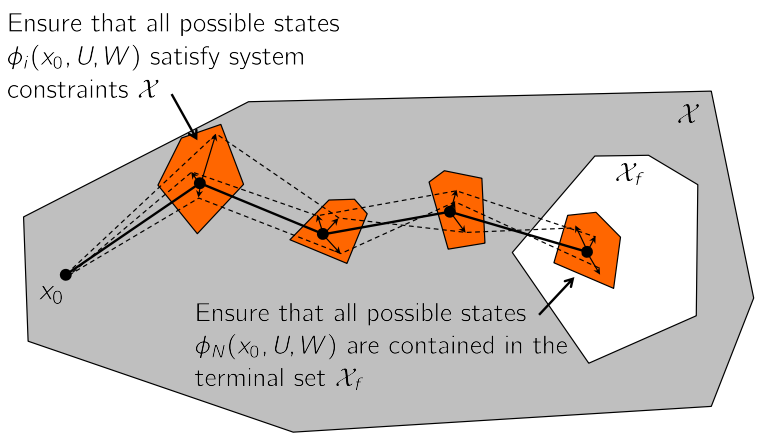
\includegraphics[width=0.7\textwidth]{images/robust_constraint_satisfaction.png}
    \caption{Robust constraint satisfaction through constraint tightening. The nominal
    trajectory is required to satisfy tighter constraints so that the entire set of possible
    disturbed states remains inside the original constraint set \(\mathcal X\). At the terminal
    time, all possible terminal states must be contained in the robust terminal set
    \(\mathcal X_f\).}
    \label{fig:robust_constraint_satisfaction}
\end{figure}

This point of view separates the MPC prediction into two parts. Over the finite horizon
\(i=0,\ldots,N-1\), the optimizer chooses the input sequence
\[
    U=\{u_0,\ldots,u_{N-1}\}
\]
and constraints are enforced explicitly on all possible disturbed predictions. At the end of the
horizon, one imposes a terminal constraint
\[
    \phi_N(x_0,U,W)\in\mathcal X_f
    \qquad
    \forall W\in\mathcal W^N,
\]
where \(\mathcal X_f\subseteq \mathcal X\) is chosen as a robust positively invariant set for the
post-horizon dynamics. In the simple open-loop construction considered here, after the horizon
one assumes no further planned input, i.e. \(u_i=0\) for \(i\geq N\), and therefore the
post-horizon system is
\[
    \phi_{i+1}=A\phi_i+w_i.
\]
If \(\mathcal X_f\) is robust positively invariant for this system and \(0\in\mathcal U\), then
once the terminal state is inside \(\mathcal X_f\), the constraints can be maintained
indefinitely despite the disturbance.

\subsubsection{Constraint tightening along the horizon}

We now derive the tightened constraints explicitly. From the linearity of the dynamics, the
uncertain state at prediction step \(i\) can be written as
\[
    \phi_i(x_0,U,W)
    =
    x_i
    +
    \sum_{j=0}^{i-1} A^j w_{i-1-j},
\]
where \(x_i\) is the nominal state obtained from
\[
    x_{i+1}=Ax_i+Bu_i,
    \qquad x_0=x(0).
\]
The goal is to ensure
\[
    \phi_i(x_0,U,W)\in\mathcal X
    \qquad
    \forall W\in\mathcal W^i.
\]
Equivalently, the set
\[
    \left\{
    x_i+\sum_{j=0}^{i-1}A^jw_{i-1-j}
    \ \middle|\
    w_0,\ldots,w_{i-1}\in\mathcal W
    \right\}
\]
must be contained in \(\mathcal X\).

Assume that the state constraint set is polyhedral,
\[
    \mathcal X=\{x\mid Fx\leq f\}.
\]
Then robust constraint satisfaction at prediction step \(i\) is equivalent to
\[
    F x_i
    +
    F\sum_{j=0}^{i-1}A^j w_{i-1-j}
    \leq f
    \qquad
    \forall W\in\mathcal W^i.
\]
For each row of \(F\), we must protect against the largest possible disturbance contribution.
Thus,
\[
    F x_i
    \leq
    f
    -
    \max_{W\in\mathcal W^i}
    F\sum_{j=0}^{i-1}A^j w_{i-1-j}.
\]
The maximization is understood row-wise. In terms of support functions, this can be written as
\[
    F x_i
    \leq
    f
    -
    h_{\mathcal W^i}
    \left(
        F\sum_{j=0}^{i-1}A^j
    \right),
\]
or, more transparently, as a tightening by the set of all possible disturbance offsets. The
important conclusion is that robust satisfaction of the original constraint can be enforced by
imposing a tighter constraint on the nominal state \(x_i\). The support-function terms depend
only on \(A\), \(F\), and \(\mathcal W\), and can therefore be precomputed offline.

\begin{theorembox}[Constraint tightening]
For the disturbed linear system
\[
    x(k+1)=Ax(k)+Bu(k)+w(k),
    \qquad w(k)\in\mathcal W,
\]
robust satisfaction of \(x_i\in\mathcal X\) can be enforced by requiring the nominal prediction
\(x_i\) to lie in a tightened constraint set. The tightening accounts for all disturbance effects
that can accumulate during the first \(i\) prediction steps.
\end{theorembox}

\subsubsection{Terminal state constraint}

The same argument applies to the terminal constraint. At the end of the horizon, we require not
only the nominal state \(x_N\), but every possible disturbed terminal state, to lie in the terminal
set:
\[
    \phi_N(x_0,U,W)\in\mathcal X_f
    \qquad
    \forall W\in\mathcal W^N.
\]
Using the same decomposition,
\[
    \phi_N(x_0,U,W)
    =
    x_N
    +
    \sum_{j=0}^{N-1} A^j w_{N-1-j},
\]
this condition is enforced by tightening the terminal constraint in exactly the same way as the
intermediate state constraints. Hence the nominal terminal state must be chosen sufficiently
inside \(\mathcal X_f\) so that all possible disturbed terminal states remain in
\(\mathcal X_f\).

\subsubsection{Set notation and disturbance reachable sets}

The previous construction can be written compactly using Minkowski sums and the Pontryagin
difference. Define the disturbance reachable set at prediction step \(i\) as
\[
    \mathcal F_i
    :=
    \bigoplus_{j=0}^{i-1} A^j\mathcal W
    =
    \mathcal W\oplus A\mathcal W\oplus\cdots\oplus A^{i-1}\mathcal W,
    \qquad
    \mathcal F_0=\{0\}.
\]
This is the set of all possible deviations between the uncertain and nominal state after \(i\)
steps. Indeed,
\[
    \phi_i(x_0,U,W)
    \in
    x_i\oplus\mathcal F_i.
\]
Therefore, the condition that every possible disturbed state lies inside \(\mathcal X\) becomes
\[
    x_i\oplus\mathcal F_i\subseteq\mathcal X.
\]
By the definition of the Pontryagin difference, this is equivalent to
\[
    x_i\in\mathcal X\ominus\mathcal F_i.
\]
Thus the robust state constraint can be written as
\[
    x_i
    \in
    \mathcal X
    \ominus
    \left(
        \bigoplus_{j=0}^{i-1}A^j\mathcal W
    \right).
\]
Similarly, the robust terminal condition is
\[
    x_N
    \in
    \mathcal X_f
    \ominus
    \mathcal F_N.
\]

The disturbance reachable sets satisfy the recursion
\[
    \mathcal F_{i+1}=A\mathcal F_i\oplus\mathcal W,
    \qquad
    \mathcal F_0=\{0\}.
\]
This recursion is useful in implementations, because the sets \(\mathcal F_i\), and therefore the
tightened constraints, can be computed offline before solving the MPC problem online.

\begin{figure}[t]
    \centering
    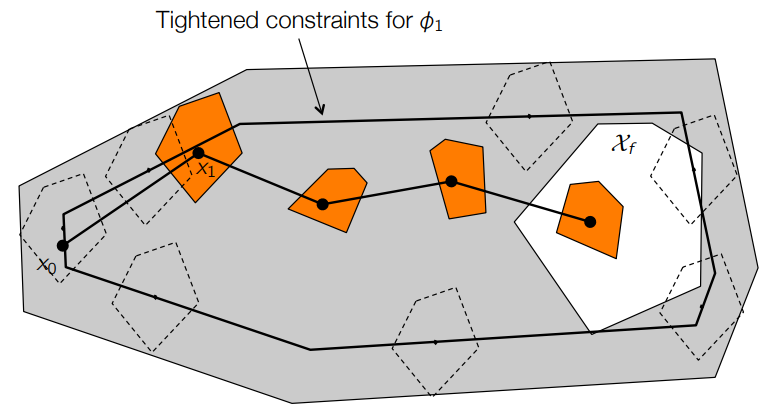
\includegraphics[width=0.7\textwidth]{images/robust_constraint_tightening_sequence.png}
    \caption{Constraint tightening along the prediction horizon. Around each nominal predicted
    state \(x_i\), the disturbance reachable set describes the possible displacement of the real
    state. If the nominal state satisfies the tightened constraint
    \(x_i\in\mathcal X\ominus\mathcal F_i\), then the whole uncertain set
    \(x_i\oplus\mathcal F_i\) remains inside the original constraint set \(\mathcal X\).}
    \label{fig:robust_constraint_tightening_sequence}
\end{figure}

\section{Robust Open-Loop MPC}

\subsection{Putting the ingredients together}

We can now combine the nominal cost, the nominal prediction dynamics, and the tightened
constraints. At time \(k\), robust open-loop MPC solves
\[
\begin{aligned}
    \min_{U}\quad
    &
    \sum_{i=0}^{N-1}\ell(x_i,u_i)+\ell_f(x_N)
    \\
    \text{subj. to}\quad
    &
    x_{i+1}=Ax_i+Bu_i,
    \qquad i=0,\ldots,N-1,
    \\
    &
    x_0=x(k),
    \\
    &
    x_i\in
    \mathcal X
    \ominus
    \left(
        \mathcal W\oplus A\mathcal W\oplus\cdots\oplus A^{i-1}\mathcal W
    \right),
    \qquad i=1,\ldots,N-1,
    \\
    &
    u_i\in\mathcal U,
    \qquad i=0,\ldots,N-1,
    \\
    &
    x_N\in
    \mathcal X_f
    \ominus
    \left(
        \mathcal W\oplus A\mathcal W\oplus\cdots\oplus A^{N-1}\mathcal W
    \right).
\end{aligned}
\]
Using the shorthand \(\mathcal F_i=\bigoplus_{j=0}^{i-1}A^j\mathcal W\), this becomes
\[
\begin{aligned}
    \min_{U}\quad
    &
    \sum_{i=0}^{N-1}\ell(x_i,u_i)+\ell_f(x_N)
    \\
    \text{subj. to}\quad
    &
    x_{i+1}=Ax_i+Bu_i,
    \qquad i=0,\ldots,N-1,
    \\
    &
    x_0=x(k),
    \\
    &
    x_i\in\mathcal X\ominus\mathcal F_i,
    \qquad i=1,\ldots,N-1,
    \\
    &
    u_i\in\mathcal U,
    \qquad i=0,\ldots,N-1,
    \\
    &
    x_N\in\mathcal X_f\ominus\mathcal F_N.
\end{aligned}
\]
Here \(\mathcal X_f\subseteq\mathcal X\) is a robust positively invariant set for the autonomous
disturbed system
\[
    x(k+1)=Ax(k)+w(k),
    \qquad w(k)\in\mathcal W.
\]

\begin{theorembox}[Robust open-loop MPC]
Robust open-loop MPC solves a nominal finite-horizon optimal control problem, but imposes
tightened state and terminal constraints. If the nominal trajectory satisfies the tightened
constraints, then every disturbed trajectory generated by \(w(k)\in\mathcal W\) satisfies the
original constraints.
\end{theorembox}

The name ``open-loop'' refers to the structure of the prediction problem. The optimizer chooses
an input sequence
\[
    U=\{u_0,\ldots,u_{N-1}\}
\]
without allowing the later inputs \(u_1,\ldots,u_{N-1}\) to depend on future disturbed states.
After solving the problem, MPC is still implemented in receding-horizon fashion:
\[
    u(k)=u_0^\star(x(k)).
\]
At the next sampling instant, the new state is measured and the optimization problem is solved
again.

\subsection{Interpretation and limitations}

The robust open-loop construction has a simple interpretation. We perform nominal MPC, but we
do not allow the nominal trajectory to approach the boundary of the true constraint set. Instead,
we keep a safety margin around it. This safety margin is exactly the disturbance reachable set
\(\mathcal F_i\). If the nominal state \(x_i\) lies in the tightened set
\(\mathcal X\ominus\mathcal F_i\), then every possible disturbed state lies in the original set
\(\mathcal X\).\\

This approach gives a systematic way to guarantee robust constraint satisfaction, but it may be
conservative. The reason is that the planned future inputs are open-loop: they cannot react to
the disturbances that will be observed in the future. The controller does re-optimize at the next
sampling instant, so feedback exists at the closed-loop level, but the prediction problem itself
does not optimize over feedback policies.\\
As a result, robust open-loop MPC can have a small feasible region, or region of attraction,
especially when the disturbance set \(\mathcal W\) is large or the horizon is long. More advanced
robust MPC schemes reduce this conservatism by explicitly introducing feedback in the prediction
model, for example through tube-based MPC. The tools developed in this chapter, namely robust
invariance, disturbance reachable sets, Pontryagin difference, and constraint tightening, are the
basic ingredients for those methods.

\section{Summary}

This chapter introduced a first robust MPC formulation for linear systems affected by bounded
additive disturbances. The main difference from nominal MPC is that a fixed input sequence no
longer generates a single predicted trajectory. Instead, it generates a family of possible
trajectories, one for each admissible disturbance sequence.\\

The cost can be treated in different ways. One may minimize an expected cost, a worst-case
cost, or, as in this lecture, a nominal cost. In the formulation considered here, robustness is not
introduced through the objective, but through the constraints.\\
The key mechanism is constraint tightening. Since the uncertain state satisfies
\[
    \phi_i(x_0,U,W)\in x_i\oplus\mathcal F_i,
    \qquad
    \mathcal F_i=\bigoplus_{j=0}^{i-1}A^j\mathcal W,
\]
robust satisfaction of \(x_i\in\mathcal X\) is guaranteed by imposing
\[
    x_i\in\mathcal X\ominus\mathcal F_i
\]
on the nominal prediction. The same construction applies to the terminal constraint, leading to
\[
    x_N\in\mathcal X_f\ominus\mathcal F_N.
\]
Robust open-loop MPC therefore solves a nominal finite-horizon optimal control problem with
tightened constraints. This guarantees constraint satisfaction for all admissible disturbances,
but it can be conservative because future inputs are planned open-loop. This motivates the
feedback-based robust MPC methods introduced next.